\section{Лекция 3 -- 2024-03-01 -- }

\begin{theorem}
  $\mathcal{A} = \left\{ S_1, S_2, \dots, S_{m_1} \right\} \subset S = \left\{ S_1, \dots, S_m \right\} $
\end{theorem}

% TODO дописать начало лекции до 



\begin{theorem}
  $\mu_k = M(M^A | \xi_0=k)$, $\mu_k = \mu_k^A$ -- наименьшее наотрицателььное решение системы:
  \[
    \begin{cases}
      \mu_k = 0, & S_k \in \mathcal{A} \\
      \mu_k = 1 + \sum_{j={m_1+1}}^m p_{kj} \mu_j, &S_k \notin \mathcal{A}.
    \end{cases}
  \]
\end{theorem}


\begin{ex}[продолжение]
  \begin{align*}
    \mu_0 &= 0, \\
    \mu_k &= 1 + q \mu_{k+1} + p \mu_{k+1}, \\
    \mu_k &= A \cdot 1^k + B \left( \dfrac{q}{p} \right)^k + \mu_k^{\text{ч}}, \\
    \mu_k^{\text{ч}} &= \begin{cases}
      A_1 \alpha^k, &\text{если $\alpha$ не является корнем характеристического} \\
      A_1 k \alpha^k, &\text{является однократным корнем} \\
      A_1 k^2 \alpha^k, &\text{является двукратным корнем}
    \end{cases} = \begin{cases}
      A_1 k, & q \neq p \\
      A_1 k^2, & q = p
    \end{cases} 
  \end{align*}

  Если $q \neq p$, то 
  \[
    \mu_k^\text{ч} = A_1 k, \quad
    A_1 k = 1 + q A_1 (k-1) + p A_1 (k+1)
    \Rightarrow
    A_1 k \cdot 0 = 1 - qA_1 + p A_1
    \Rightarrow
    A = \dfrac{k}{q-p}
  \]
  Тогда при $p>\dfrac{1}{2}$:
  \[
    \mu_k = A + B \left( \dfrac{q}{p} \right)^k + \dfrac{k}{q-p}
  \]
  Причём $\mu_0 = A + B = 0 \Rightarrow A = -B$
  \[
    \mu_k = A \left( 1 - \left( \dfrac{q}{p} \right)^k \right) + \dfrac{k}{q-p} = \infty
  \]
  Равно бесконечности, так как второе слагаемое при $k \to \infty$ сколь угодно большое по модулю,
  но меньше нуля, а первое слагаемое стремиться к константе $A$. Поэтому, чтобы не было отрицательным
  надо чтобы $A = \infty$.

  Если $p < 1/2$:
  \[
    \mu_k = A + B \left( \dfrac{q}{p} \right)^k + \dfrac{k}{q-p} = B \left( \left( \dfrac{q}{p} \right) ^k - 1 \right) + \dfrac{k}{q-p} \geqslant \dfrac{k}{q-p}
  \]

  Если $p = q$:
  \begin{align*}
    \mu_k &= A + Bk + \mu_k^\text{ч} = A + Bk + A_1 k^2, \\
    \cancel{A_1 k^2} &= 1 + q A_1 (\cancel{k^2} - 2k+1) + pA_1 (\cancel{k^2} + 2k + 1), \\
    \Leftrightarrow A_1 &= -1.
  \end{align*}

  Ищем наименьшее неотрицательное решение. $\mu_k = A + Bk - k^2$, Квадрат рано или поздно сделает
  это выражение отрицательным, поэтому наименьшее неотрицатьельное решение $\mu_k = \infty$.

  Время вырождения получилось бесконечным, но вероятность вырождения равна единице. То
  есть выродится, но просто когда-то.

  Можно провести аналогию с рядами. Если $P(\xi = k) = \dfrac{1}{k}$, то математическое ожидание
  расходится, вот это очень похожая история.
\end{ex}

\subsection{Марковская цепь с непрерывным временем}

$\mathcal{S} = \left\{ S_1, S_2, \dots, S_m \right\}$

\begin{definition}
  Если $P(\xi_{t+\Delta t} = j | \xi_t = i) = p_{ij}(t, \Delta t)$ не зависит от значений $\xi_s$, 
  $s \in [0, t)$.

  Более того, если $p_{ij}(t, \Delta t) = \lambda_{ij}(t) \Delta t + o(\Delta t)$, 
  то $\lambda_{ij} $ называется \emph{интенсивностью} переходной вероятности
  из $i$ в $j$ в момент времени $t$.

  Если $\lambda_{ij} (t) = \lambda_{ij}$ не зависит от $t$, то МЦ называется \emph{однородной}.
\end{definition}

\begin{ex}[Пуассоновский поток событий]
  \[
    \begin{cases}
      P(\text{за $\Delta t$ случается 1 событие}) = \lambda \Delta t + o(\Delta t), \\
      P(\text{за $\Delta t$ случается больше 1 события}) = o(\Delta t)
    \end{cases}
  \]
  -- однородная марковская цепь с интенсивностью $\lambda$.

  % TODO рисунок числовая прямая

  Граф этой МЦ:
  \begin{figure}[h!]
    \centering
    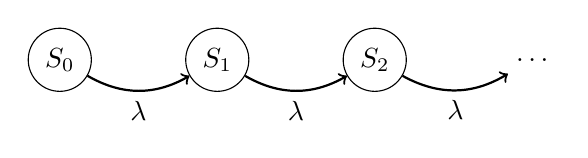
\begin{tikzpicture}
      \begin{scope}[every node/.style={fill=white,circle,draw=black}]
        \node (S_0) at (0,0) {$S_0$};
        \node (S_1) at (2,0) {$S_1$};
        \node (S_2) at (4,0) {$S_2$};
        \node[draw=white] (S_dots) at (6,0) {$\dots$};
      \end{scope}
    
      \begin{scope}[->, every edge/.style={draw=black,thick}]
        \path (S_0) edge [bend right=30] node[below] {$\lambda$} (S_1);
        \path (S_1) edge [bend right=30] node[below] {$\lambda$} (S_2);
        \path (S_2) edge [bend right=30] node[below] {$\lambda$} (S_dots);
      \end{scope}
    \end{tikzpicture}
  \end{figure}

  Причём подписи у рёбер графа -- не вероятности, а интенсивности, поэтому могут
  быть больше единицы.

  \[
    P(\xi_{t+\Delta t} = j | \xi_t = i) = \begin{cases}
      \lambda \Delta t, & j = i+1 \\
      0 & j \neq i+1, j \neq i \\
      1-\lambda \Delta t + o(\Delta t), & j =1
    \end{cases}
  \]
\end{ex}

\begin{theorem}
  Пусть $\lambda_{ij}(t)$ -- интенсивности вероятности перехода. Пусть
  $p(t) = (p_0(t), p_1(t), \dots, p_m(t))^T$
  -- вектор вероятностей состояний в момент $t$.
  \[
    \Lambda = (\lambda_{ij}), \lambda_{ii} = - \sum_{j\neq i} \lambda_{ij} 
  \]
  Эту сумму (без минуса) иногда называют интенсивностью истекающего потока.

  Тогда
  \[
    p'(t) = \Lambda^T(t) p(t) 
    \leftrightarrow
    p'^T(t) = p(t)^T \Lambda(t)
    \leftrightarrow
    p_k'(t)
    = \sum_{i=1, i\neq k}^m \lambda_{ik}(t) p_{i}(t)
      - \sum_{i=1, i\neq k}^m \lambda_{ki}(t) p_k(t)
  \]
  такая система называется системой дифференциальных уравнений Колмогорова.
\end{theorem}
\begin{proof}
  \begin{multline*}
    p_k(t+\Delta t) = P(\xi_{t+\Delta t} = k)
    = \sum_{j=1}^m P(\xi_{t+\Delta t} = k | \xi_t = j) \cdot P(\xi_t = j) = \\
    = \sum_{j=1, j \neq k}^m \lambda_{ij}(t) \Delta t \cdot p_j(t)
      + P(\xi_{t+\Delta t} = k | \xi_t = k) \cdot P(\xi_t = k) + o(\Delta t) = \\
    = \sum_{j=1, j \neq k}^m \lambda_{ij}(t) \Delta t \cdot p_j(t)
      + \left( 1 - \sum_{j\neq k} \lambda_{kj}(t) \Delta t\right)  P(\xi_t = k) + o(\Delta t) = \\
  \end{multline*}

  \[
    p_k(t+\Delta t) - p_k(t) = \sum_{j\neq k} \lambda_{jk}(t) \Delta t p_j(t) - \lambda_{kk} (t) p_k(t)
    \Rightarrow
    p_k'(t) = \sum_{j\neq k} \lambda_{jk} (t) p_j(t) - \lambda_{kk}(t) p_k(t)
  \]
  (поделили на $\Delta t$ и устремили к 0).
\end{proof}

\begin{ex}[Пуассоновский поток]
  Пусть в начальный момент времени находились в состоянии $S_0$:
  \[
    p(0) = (1, 0, 0, \dots)^T
  \]

  \begin{figure}[h!]
    \centering
    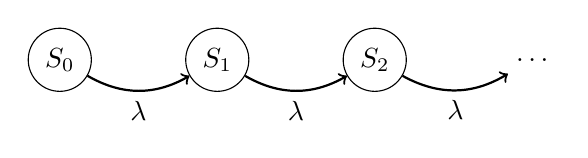
\begin{tikzpicture}
      \begin{scope}[every node/.style={fill=white,circle,draw=black}]
        \node (S_0) at (0,0) {$S_0$};
        \node (S_1) at (2,0) {$S_1$};
        \node (S_2) at (4,0) {$S_2$};
        \node[draw=white] (S_dots) at (6,0) {$\dots$};
      \end{scope}
    
      \begin{scope}[->, every edge/.style={draw=black,thick}]
        \path (S_0) edge [bend right=30] node[below] {$\lambda$} (S_1);
        \path (S_1) edge [bend right=30] node[below] {$\lambda$} (S_2);
        \path (S_2) edge [bend right=30] node[below] {$\lambda$} (S_dots);
      \end{scope}
    \end{tikzpicture}
  \end{figure}

  \[
    \begin{cases}
      p_0' = -\lambda p_0, \\
      p_1' = \lambda p_0 - \lambda p_1, \\
      \dots \\
      p_k' = \lambda p_{k-1} - \lambda p_k
    \end{cases}
  \]
  -- с плюсом всё что втекает, с минусом всё что вытекает.

  Операционно решим:
  \[
    p_k(t) \risingdotseq \tilde p_k(s) 
    \Rightarrow
    p_k'(t) \risingdotseq s \tilde p_k(s) - p_k(0)
  \]

  \[
    \begin{cases}
      s \tilde p_0 - 1 = - \lambda \tilde p_0, \\
      s \tilde p_1 = \lambda \tilde p_0 - \lambda \tilde p_1, \\
      \dots
      
    \end{cases}
    \Rightarrow
    \begin{cases}
      \tilde p_0 = \dfrac{1}{s+\lambda} \fallingdotseq e^{-\lambda t}, \\
      \tilde p_1 = \dfrac{\lambda \tilde p_0}{s+\lambda} = \dfrac{\lambda}{(s+\lambda)^2}
        \fallingdotseq \lambda t e^{-\lambda t}, \\
      \dots \\
      \tilde p_{k+1} = \dfrac{\lambda \tilde p_k}{s+\lambda}=\dfrac{\lambda^{k+1}}{(s+\lambda)^{k+2}}
        \fallingdotseq e^{-\lambda t}, \\

    \end{cases}
  \]

  \[
    p(t) = \left( e^{-\lambda t}, \lambda t e^{-\lambda t}, \dots, \dfrac{(\lambda t)^k}{k!} e^{-\lambda t}, \dots \right)^T.
  \]
\end{ex}

Финальные вероятности находятся по формуле:
\[
  \lim_{t\to +\infty} p_n(t) = \lim_{j \to 0} s \tilde p(s)
\]
(по теореме из операционного исчисления)
